\documentclass[a4paper]{article}

\usepackage[top=1in, bottom=1.25in, left=1in, right=1in]{geometry}
\usepackage{media9}
\usepackage[english]{babel}
\usepackage[utf8]{inputenc}
\usepackage{amsmath}
\usepackage{graphicx}
\usepackage{subfigure}
\usepackage[colorinlistoftodos]{todonotes}

\title{Learning from $A^*$ by Applying a Convolutional Neural Network}

\author{Saniea Akhtar, Hendrik Vloet}

\date{\today}

\begin{document}
\maketitle
\section{Introduction}

\subsection{Short Recap of $A^*$}

$A^*$ is an informed search method that combines the best of a greedy search with the uniform-cost search. It is an estimation method and uses 3 functions in order to determine which node, i.e. action it should take next. Furthermore it has some specific properties, that are shortly recapped in the following list\footnote{Information, equations and definitions are taken from the lecture 'Foundations of A.I.'}:
\begin{itemize}
\item $g(n)$: actual cost from the initial state to current state $n$
\item $h(n)$: estimated cost from current state $n$ to the nearest goal state (also called 'heuristic')
\item $f(n) = g(n)+h(n)$: the estimated cost of the cheapest solution through $n$
\item $h^*(n)$: the actual (normally unknown) cost of the optimal path from state $n$ to the nearest goal state
\item Admissibility: A heuristic is admissible if the chosen heuristic estimates the costs of a state to the nearest goal state less or equal to the actual costs, i.e. $h(n) \leq h^*(n) \forall n$
\item Completeness: $A^*$ will find a solution (if it exists) if every node has a finte number of successor nodes and there exists a positive constant $\delta > 0$ such that every step has at least cost $\delta$
\item Complexity: 
\begin{itemize}
\item exponential in time and memory
\item if only one goal state exists and the search graph is a tree, then a sub-exponential number of nodes will be expanded: $\vert h^*(n) - h(n) \vert \leq O(log(h^*(n)))$
\end{itemize}
\item Consistency: $h$ is consistent if and only if for all actions $a$ leading from state $s$ to $s'$:$h(s)-(h(s')) \leq c(a)$, where $c(a)$ denotes the cost of action $a$. C
\item Iterative Deepening $A^*$: This is a variant of $A^*$, it is used in our environment as well since the teaching planner gets cut-off after it exceeded a certain amount of steps.
\end{itemize}


\clearpage
\section{Tasks}
This section will be divided into two parts: in part one we consider the tasks given by the exercise sheet and in party two we consider additional experimental stuff we played around with.

\subsection{\textbf{Default Tasks}}

A summary of how different history lengths affect the agent's performance is given in Table 1. Following is a short assessment of the same results. A tensorboard picture of the used setup can be found in figure \ref{fig:tb_default}
\begin{figure}[hbpt!]
\centering
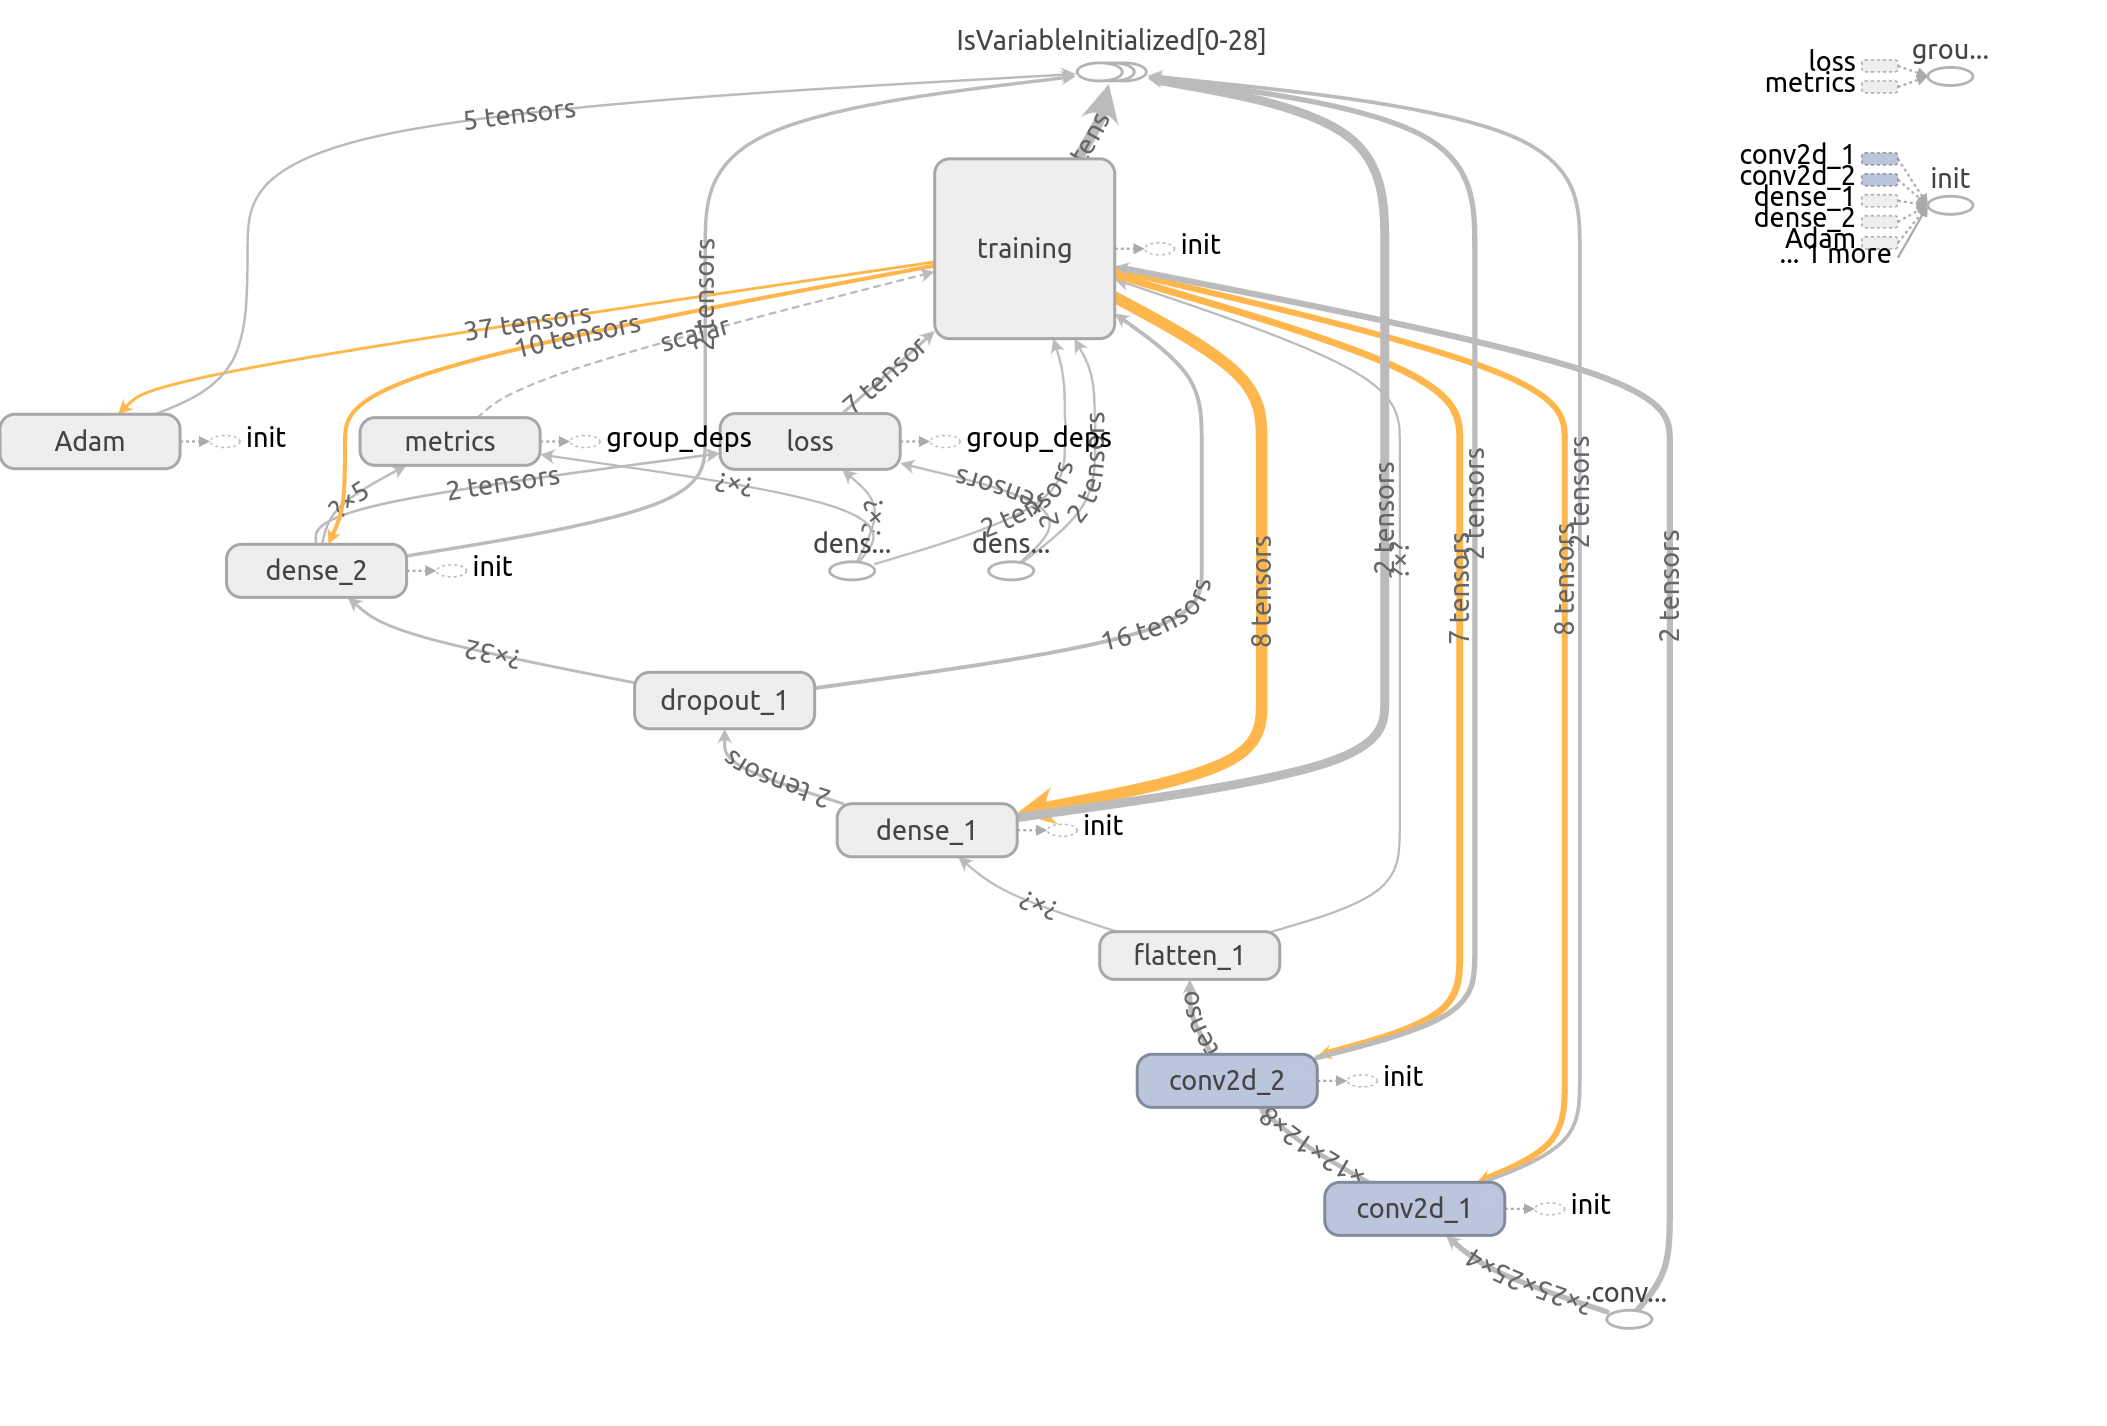
\includegraphics[height=8cm, width=\textwidth]{default_setup_graph.png}
\label{fig:tb_default}
\caption{Default Setup for performing the tasks}
\end{figure}

The following diagrams show how well our agent did perform in general on the default map.\\
We used 20 epochs for training, a learning rate of $0.001$ and the ADAM optimizer (the according .csv files can be found in the report directory)
For comparison: The random behavior agent did score a test accuracy of 10\%, as expected.

\begin{minipage}[t]{0.45\textwidth}
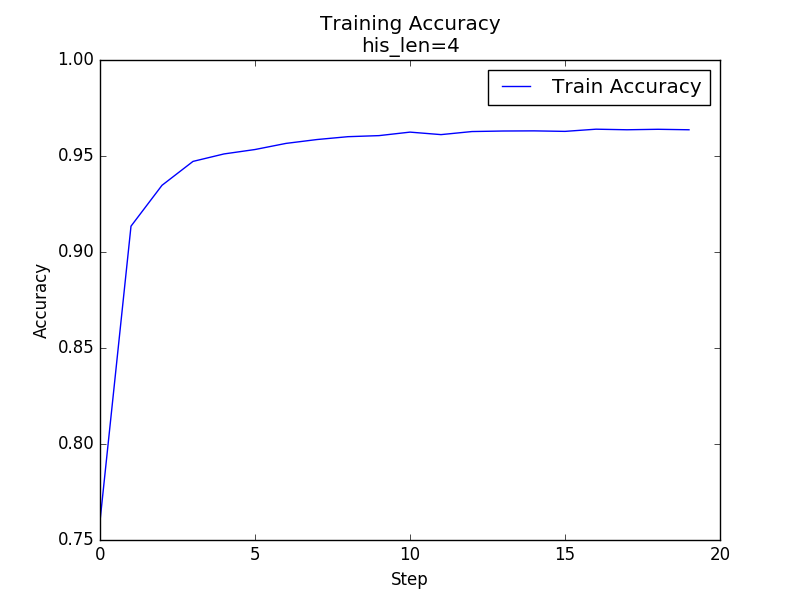
\includegraphics[height=3.5cm,width=\textwidth]{train_acc_default.png}
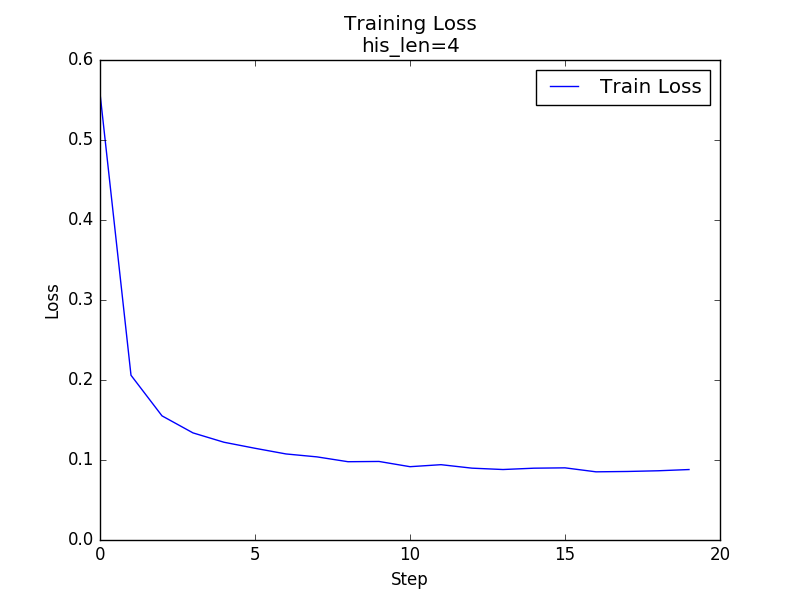
\includegraphics[height=3.5cm,width=\textwidth]{train_loss_default.png}
\end{minipage}
\begin{minipage}[t]{0.45\textwidth}
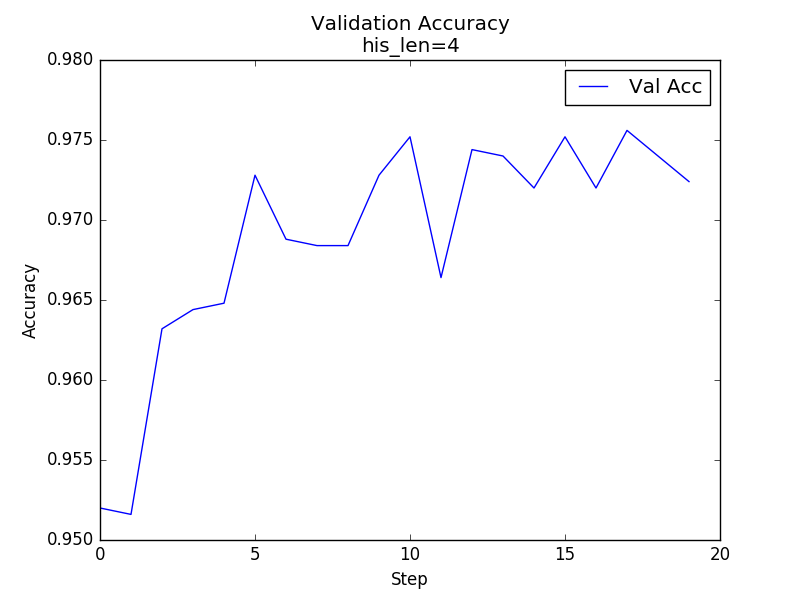
\includegraphics[height=3.5cm,width=\textwidth]{val_acc_default.png}
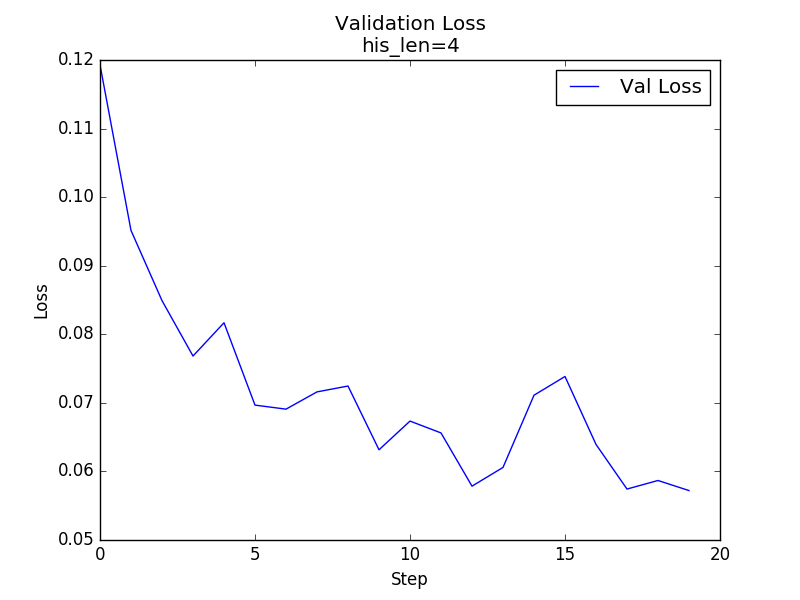
\includegraphics[height=3.5cm,width=\textwidth]{val_loss_default.png}

\end{minipage}





\clearpage
\textbf{History Length Comparison Table}\\
\\
\begin{tabular}{|c|c|c|c|c|c|c|c|}
\hline 
Hist Len & Train Loss & Train Acc & Val Loss & Val Acc & Train Time (m) & Test Acc & Avg Steps \\ 
\hline 
1 & 0.2614 & 0.8795 & 0.2217 & 0.92 & 0.2528 & 0.8 & 20 \\ 
\hline 
2 & 0.1854 & 0.9170 & 0.1395 & 0.932 & 0.2537 & 0.967 & 16.96 \\ 
\hline 
3 & 0.2054 & 0.9126 & 0.1164 & 0.944 & 0.2579 & 0.966 & 16.9 \\ 
\hline 
4 & 0.1896 & 0.9169 & 0.2406 & 0.96 & 0.2579 & 0.966 & 20.45 \\ 
\hline 
5 & 0.2067 & 0.9096 & 0.0958 & 0.9569 & 0.2647 & 1 & 15.9 \\ 
\hline 
6 & 0.1961 & 0.9164 & 0.1167 & 0.9560 & 0.2635 & 1 & 20.04 \\ 
\hline 
7 & 0.2011 & 0.9197 & 0.1513 & 0.948 & 0.2708 & 1 & 19.19 \\ 
\hline 
8 & 0.1575 & 0.9306 & 0.1458 & 0.9520 & 0.2749 & 0.95 & 22.46 \\ 
\hline 
9 & 0.2238 & 0.9098 & 0.2118 & 0.9440 & 0.2910 & 1 & 21.39 \\ 
\hline 
10 & 0.2287 & 0.9074 & 0.2275 & 0.928 & 0.2809 & 0.95 & 23.05 \\ 
\hline
\end{tabular} 


\begin{itemize}

\item \textbf{History Length Variation}\\
Changes in the length of history had clear affects on the performance of the agent. The default length of history was set at 4. Reducing the history to the lowest possible value of 1, immediately resulted in a loss of accuracy from 96$\%$ to 83$\%$. Since the agent no longer had any record of the steps taken beyond the last one, it was more likely to repeat the same steps and thus less likely to reach the target in the the maximum number of steps.

After observing the affects of changing the history to 1, we swept over a history length from 1 till 10. As can be seen from the training accuracy and validation accuracy, history lengths longer than 8 appear to be overfitting the data which is why there is big difference between the validation and training accuracy. Overall, changing history beyond 8, doesn't have a significant impact on the performance and would be the optimum history length.


\item \textbf{Performance in Local View}\\
By default, the agent was not able to have a view of the entire map; only a 5x5 field of view window was available to the agent. Based on the training data generated from the \textit{$get\_data.py$} script, the agent was able to reach the target location with a relatively high accuracy. On average, the success rate of the agent lied between 96$\%$ to 100$\%$. 

We tried to change the POB size but also had to realize that obiously only odd numbers would work, but we also had to include '1' padding of the outer walls, because if the POB is higher than default, the agent would look through the outer walls and produce the following error message:

\begin{figure}[hbpt!]
\centering
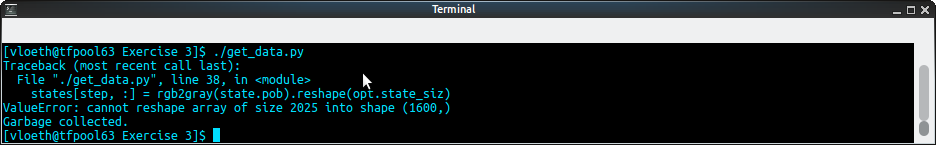
\includegraphics[height=2cm, width=\textwidth]{error_pob.png}
\label{fig:pob_error}
\end{figure}
\begin{center}

We used 3200 samples for the following experiments with the POB.
\begin{tabular}{|c|c|c|c|c|c|}
\hline 
history length & POB & Train Acc & Val Acc & Success Rate & Avg Steps \\ 
\hline 
2 & 3x3 & 77\% & 82\% & 78.2\% & 21.6 \\ 
\hline 
2 & 5x5 & 81\% & 94\% & 83\% & 20.7 \\ 
\hline 
2 & 7x7 & 82\% & 88\% & 87\% & 20.9 \\ 
\hline
\hline 
4 & 3x3 & 83\% & 80\% & 90.1\% & 22.6 \\ 
\hline 
4 & 5x5 & 83\% & 89\% & 95\% & 22.5 \\ 
\hline 
4 & 7x7 & 87\% & 92\% & 96\% & 17.7 \\ 
\hline 
\end{tabular} 
\end{center}

So, as expected,increasing the field of view results in an improved success rate. In conclusion it is valid to say that the more the agent can see of its environment, the better it can orientate. We will keep that in mind, when we try to generalize well on new unseen maps.


% We tried to change the field of view of the agent to see how it affected the performance, however for some very strange reason, we were unable to generate any training data for the agent with an increased window size. At the time of writing this report, we are still attempting to understand why the script is unable to work with a changed window size since the variation seems to trivial.





\item \textbf{New Target Location After Training}\\
After training the agent for the default target location of [12,11], for testing, we changed the target location to some other valid point. After this change, the performance of the agent solely depending upon the starting point of the simulation. If the agent was able to start at a point relatively close to target location, it was successful in reaching its goal, otherwise it would frequently reach the max limit of steps without reaching the target location, because it tries to reach the old target location what it has been trained upon.

The reason the agent failed to perform as it should have is because it is only able to have a limited view of the environment. Since the target is now placed at a point the agent has never seen or visited before, it is unable to process that the target location has changed and therefore, keeps trying to return to the same position as used in the training sessions. One way to overcome this obstacle would be to give the agent the full of view of the environment. That way, it can become aware of the new target location from the start and plan its path accordingly. However, while it increases the efficiency of the agent, giving it a view of the full environment renders the whole process of generating data and training the agent rather redundant since a simple $A^*$ algorithm will be able to achieve the same result.\\
\begin{minipage}[t]{0.45\textwidth}
\flushleft{Old Target.\\ Success Rate 100\% with 18 steps on average}
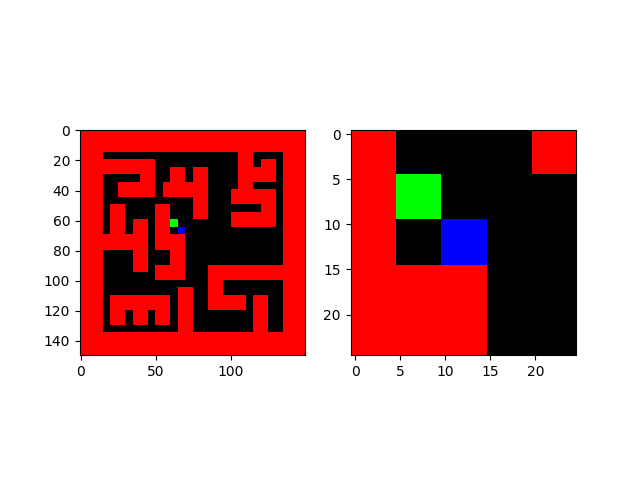
\includegraphics[height=3.5cm,width=\textwidth]{map_a_old_target.png}
\end{minipage}
\hfill
\begin{minipage}[t]{0.45\textwidth}
\flushleft{New target location.\\ Success Rate 18\% with 43.4 steps on average}
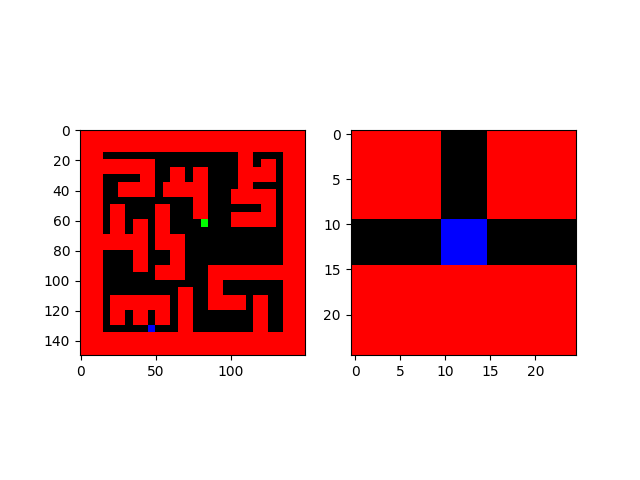
\includegraphics[height=3.5cm,width=\textwidth]{map_a_new_target.png}
\end{minipage}

\item \textbf{New Map After Training}\\
More or less the same result was expected from the agent as a result of changing the map after training. If the game initialized at a point close to the target point on the new map, the agent would be able to reach the target, mostly out of luck. But other than that, the agent was mostly not very successful.\\

In the folder of the report should be a .mkv video file, with a recorded screen of testing the agent with a current map and then changing the map, but keeping the target position(file:$change\_map.mkv$)

Another point that had to be kept in mind while making this change is that the target location of the training map, might not be a valid target location in the testing map. If that is the case, then the "target" of the agent would be inside a wall, and the no matter what the other training parameters would be, it would not be able to achieve success.
\clearpage
\item \textbf{Stuck State}\\
Sometimes the agent got stuck in front of a wall and always moves up and down, getting stuck. In that case it will terminate after the early\_step\_size is exceeded. This can happen if the field of view of the agent looks similar to the goal position and the agent basically thinks it has to be in the goal position. Increasing history length reduces this effect, though. An Example can be found in figure \ref{fig:stuck_state}
\begin{figure}[hbpt!]
\centering
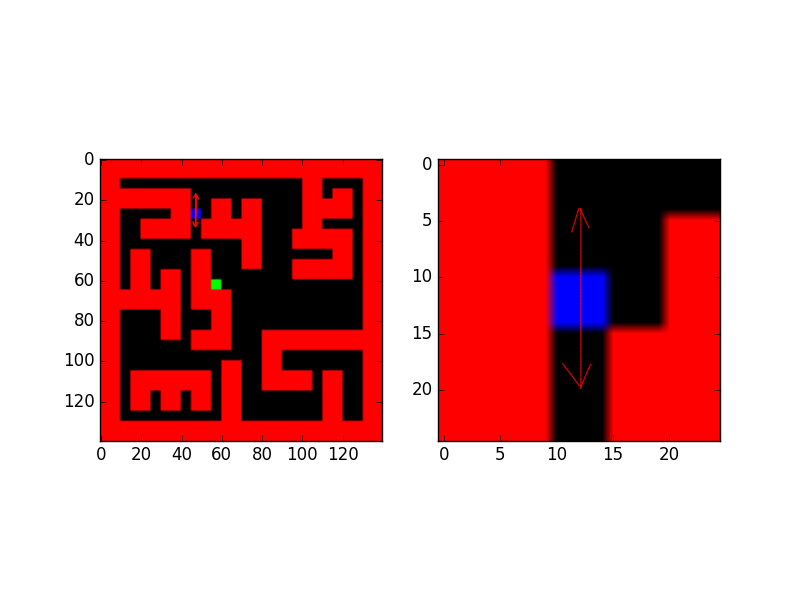
\includegraphics[width=0.8\textwidth, height=0.4\textwidth]{stuck_state.png}
\label{fig:stuck_state}
\caption{Example of a stuck state for the agent}
\end{figure}


\item \textbf{Suggestions about better Generalization}\\
Generalization is a critical point in this setup, because the environment of the agent is only partially observable, thus rendering the environment into a POMD (partially observable markov decision process). So here a few ideas of how to make improvements to the generalization ability of the agent or stating why this particular idea would not work:
\begin{itemize}
\item \textbf{History Length}: Increasing the history length does not necessarily bring improvements to the performance. This can be observed in the history length comparison table.
\item \textbf{Train on many maps:} This would also not work, because the more we train on different maps, the more the behavior would randomize and eventually perform equal or worse than a weak learn(50\% accuracy)
\item \textbf{Increasing Field of View:} This could actually work. If the agent is more aware of what his environment looks like, then he is able to generalize better on unseen data, i.e. new maps.

\begin{minipage}[t]{0.3\textwidth}
\center{Map A old target location}
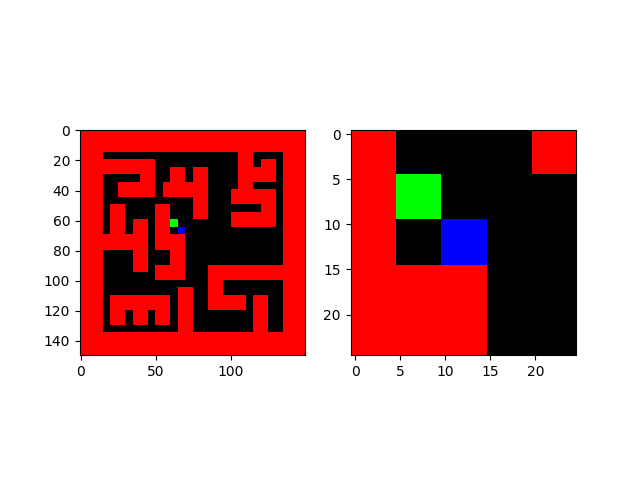
\includegraphics[height=3.5cm,width=\textwidth]{map_a_old_target.png}
\end{minipage}
\begin{minipage}[t]{0.3\textwidth}
\center{Map B old target location}
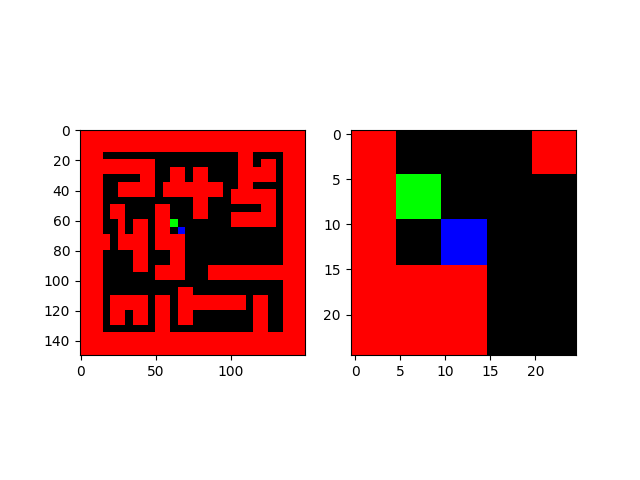
\includegraphics[height=3.5cm,width=\textwidth]{map_b_old_target.png}
\end{minipage}
\begin{minipage}[t]{0.3\textwidth}
\center{Map B new target location}
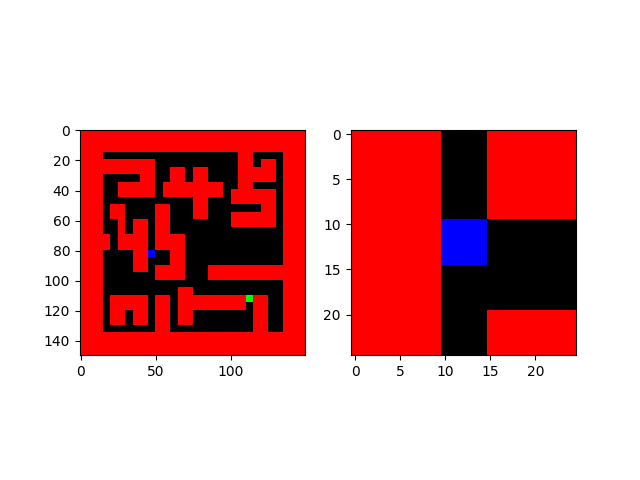
\includegraphics[height=3.5cm,width=\textwidth]{map_b_new_target.png}
\end{minipage}

So in order to check if an increased field of view would increase the success rate on a unseen new map with a new target location, we trained the agent with a field of view of 7x7 (in the picture above is a POB of 5x5 shown), a history length of 15 and a training data set of 16000 samples. \\
\begin{center}
\begin{tabular}{|c|c|c|}
\hline 
Map & Sucess Rate & Avg Steps \\ 
\hline 
Map A old Target & 100\% & 21.77 \\ 
\hline 
Map B old Target & 71\% & 28.58 \\ 
\hline 
Map B new Target & 10\% & 46 \\ 
\hline 
\end{tabular} 
\end{center}

So, making the field of view larger improves the generalization in case we are just changing the map but not the target position. The agent still remembers how to get to the target but has now other obstacles to overcome. Not the same can be said over changing the target position as well, then it will just stumble upon the target by accident, depending on the initial position of the agent.

But enlarging the field of view make the necessity of an agent that can learn somewhat pointless, because if I have full vision of my environment (and thus of the underlying Markov Decision Process or MDP) I don't need an agent. Then I just use informed search methods like $A^*$ because it will always behave optimal, if the MDP is solvable.

\item \textbf{Introduce Reinforcement Learning methods:} Since the problem of generalize well on unseen maps is an exploration vs. exploitation problem, we could use a different policy. In this version, the agent tries to approximate the behavior of $A^*$ and thus performing 100\% exploitation, 0\% exploration. If we could shift this behavior policy ($A^*$) to act according to an $\epsilon$-greedy policy, then the agent could also learn how to explore a unknown environment. An $\epsilon$-greedy policy does not take always the action that maximizes it's reward (like the $A^*$ would do) but for certain ratio it decides whether to choose the action that maximizes it's reward or to do something random and thus explores the environment. One possible architecture for this would be a Deep Q-Learning Network (DQN)
\end{itemize}

\item \textbf{Take-Away-Message}: So we think the general take away message from this exercise is, that we can use a CNN to learn from a teacher, e.g. $A^*$ and approximate the teacher behavior pretty well. But this is just for the training map. If we want to generalize as well on new and unseen map data, then we have to use more sophisticated algorithms like TD($\lambda$), Q-Learning or DQNs. We would've liked to experiment with these new ideas, but sadly we ran out of time.
\end{itemize}

\clearpage
\subsection{Additional Experimentation}

This chapter is about experimentation with different setups and playing around a bit with the environment.

\subsection{Custom Map}
We decided to draw a funny custom map which spells out "halo I bims ein Learner vong DL her" which is considered to be a German language meme. We hope you find it also funny.\\
Of course we also generated data, trained and tested it. Picture of the map and the training performance is below.

\begin{figure}[hbpt!]
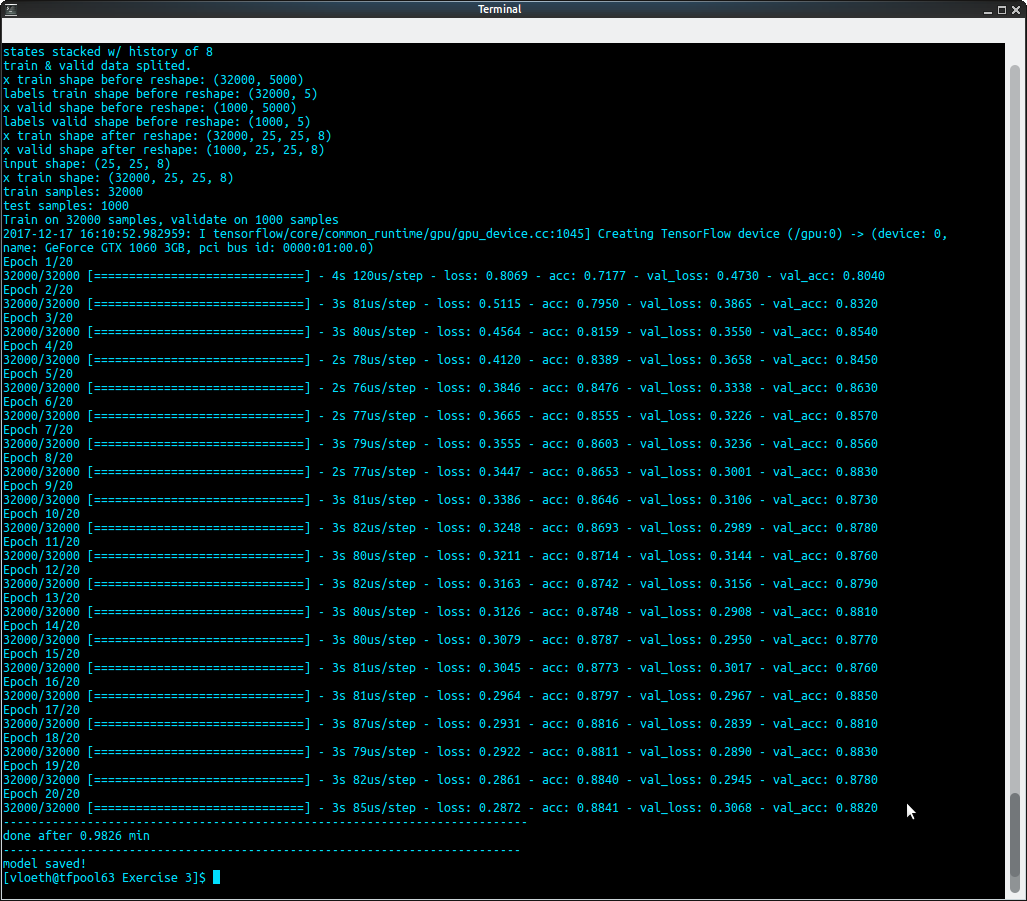
\includegraphics[height=5cm,width=\textwidth]{vong_training.png}
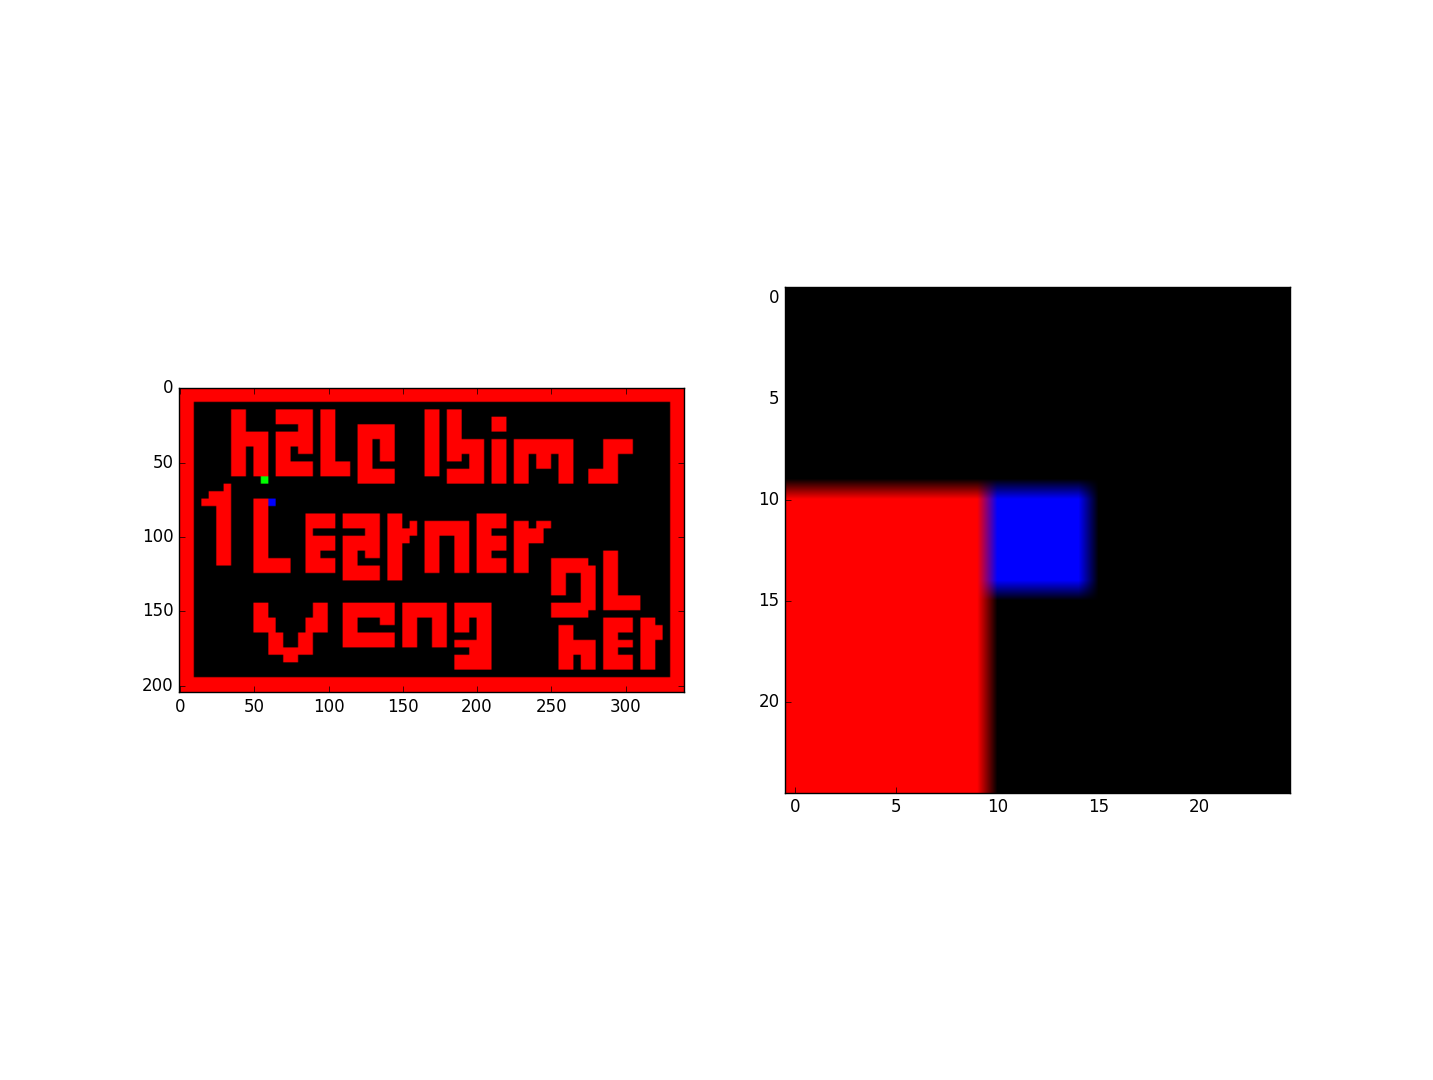
\includegraphics[height=3cm,width=\textwidth]{vong_training_map.png}


\end{figure}



Here, a video of the "vong" testing should run. If it does not, see please look up the according file in the report file directory "halo.mp4"
\begin{center}
% using a .mp4
\includemedia[width=0.6\linewidth,height=0.6\linewidth,activate=pageopen,
passcontext,
transparent,
addresource=halo.mp4,
flashvars={source=halo.mp4}
]{}{halo.mp4}

\end{center}

\subsection{Additional Architectures}

We also experimented with different architectures and you can find pictures of the graph, the training data and the testing performance below. All graphs are also included as .png files.\\
\begin{center}
\begin{tabular}{|c|c|c|}
\hline 
 Setup& Test Acc & Avg Steps \\ 
\hline 
SGD & 0.77 & 25.9 \\ 
\hline 
RMSprop & 0.85 & 24.7 \\ 
\hline 
linear output & 0 & 50 \\ 
\hline 
tanh/sigmoid & 0.96 & 17.8 \\ 
\hline 
only FC & 0.85 & 23.2 \\ 
\hline 
\end{tabular}
\end{center}


\begin{minipage}[t]{0.45\textwidth}
\flushleft{Playing with SGD}
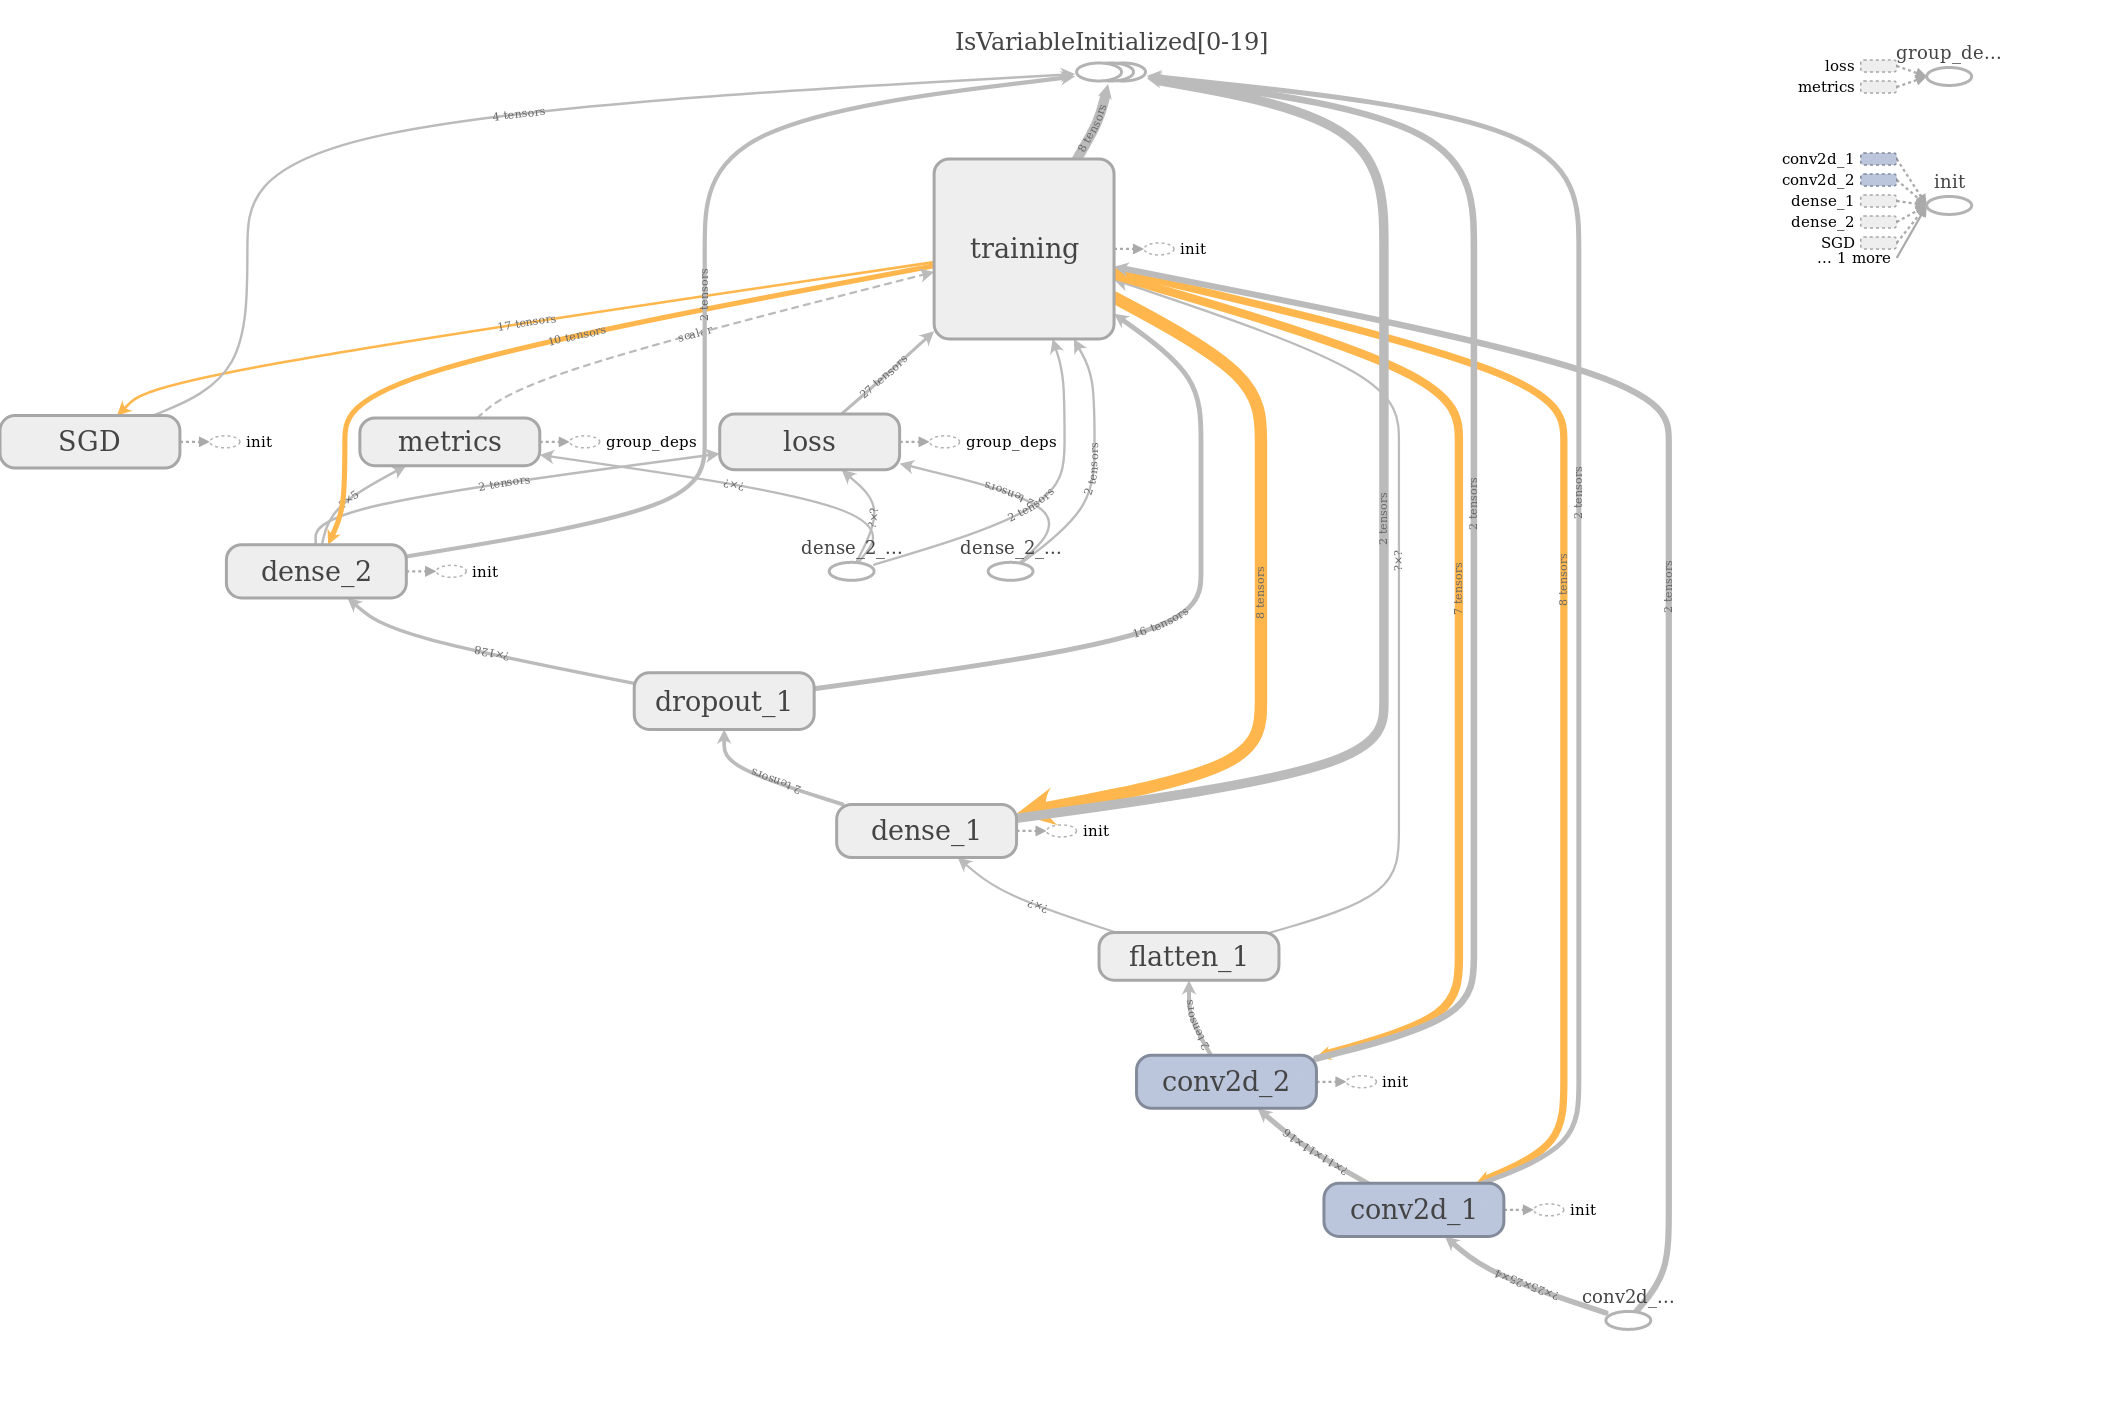
\includegraphics[height=3.5cm,width=\textwidth]{sgd_graph.png}
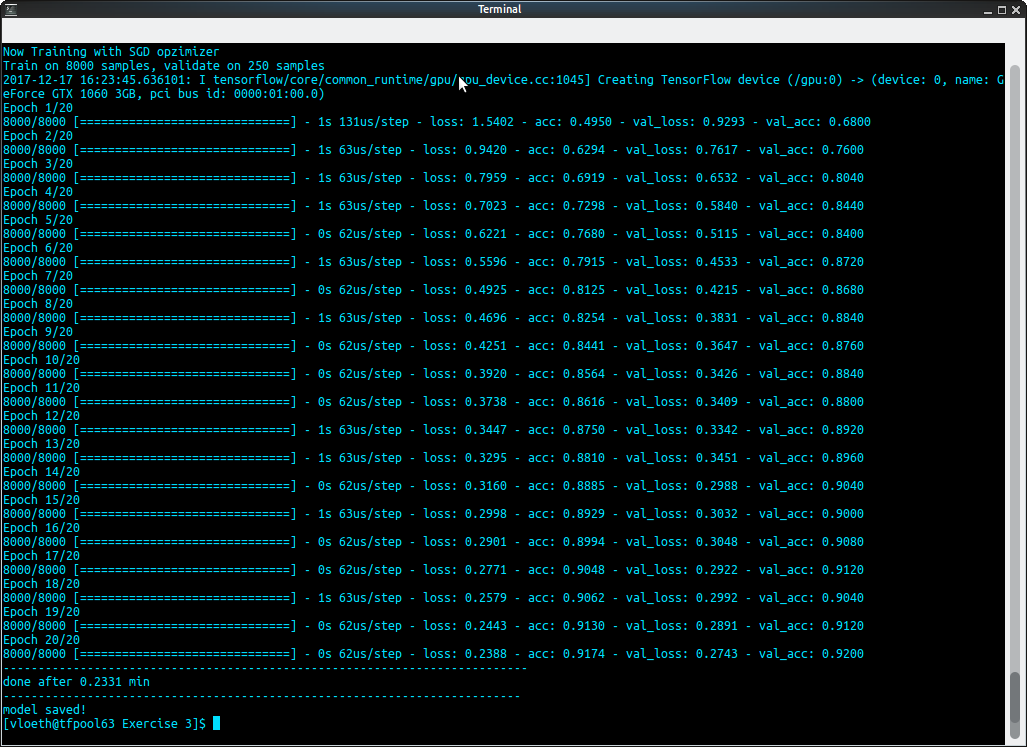
\includegraphics[height=3.5cm,width=\textwidth]{sgd_training.png}
\end{minipage}
\hfill
\begin{minipage}[t]{0.45\textwidth}
\flushleft{Playing with RMSprop}
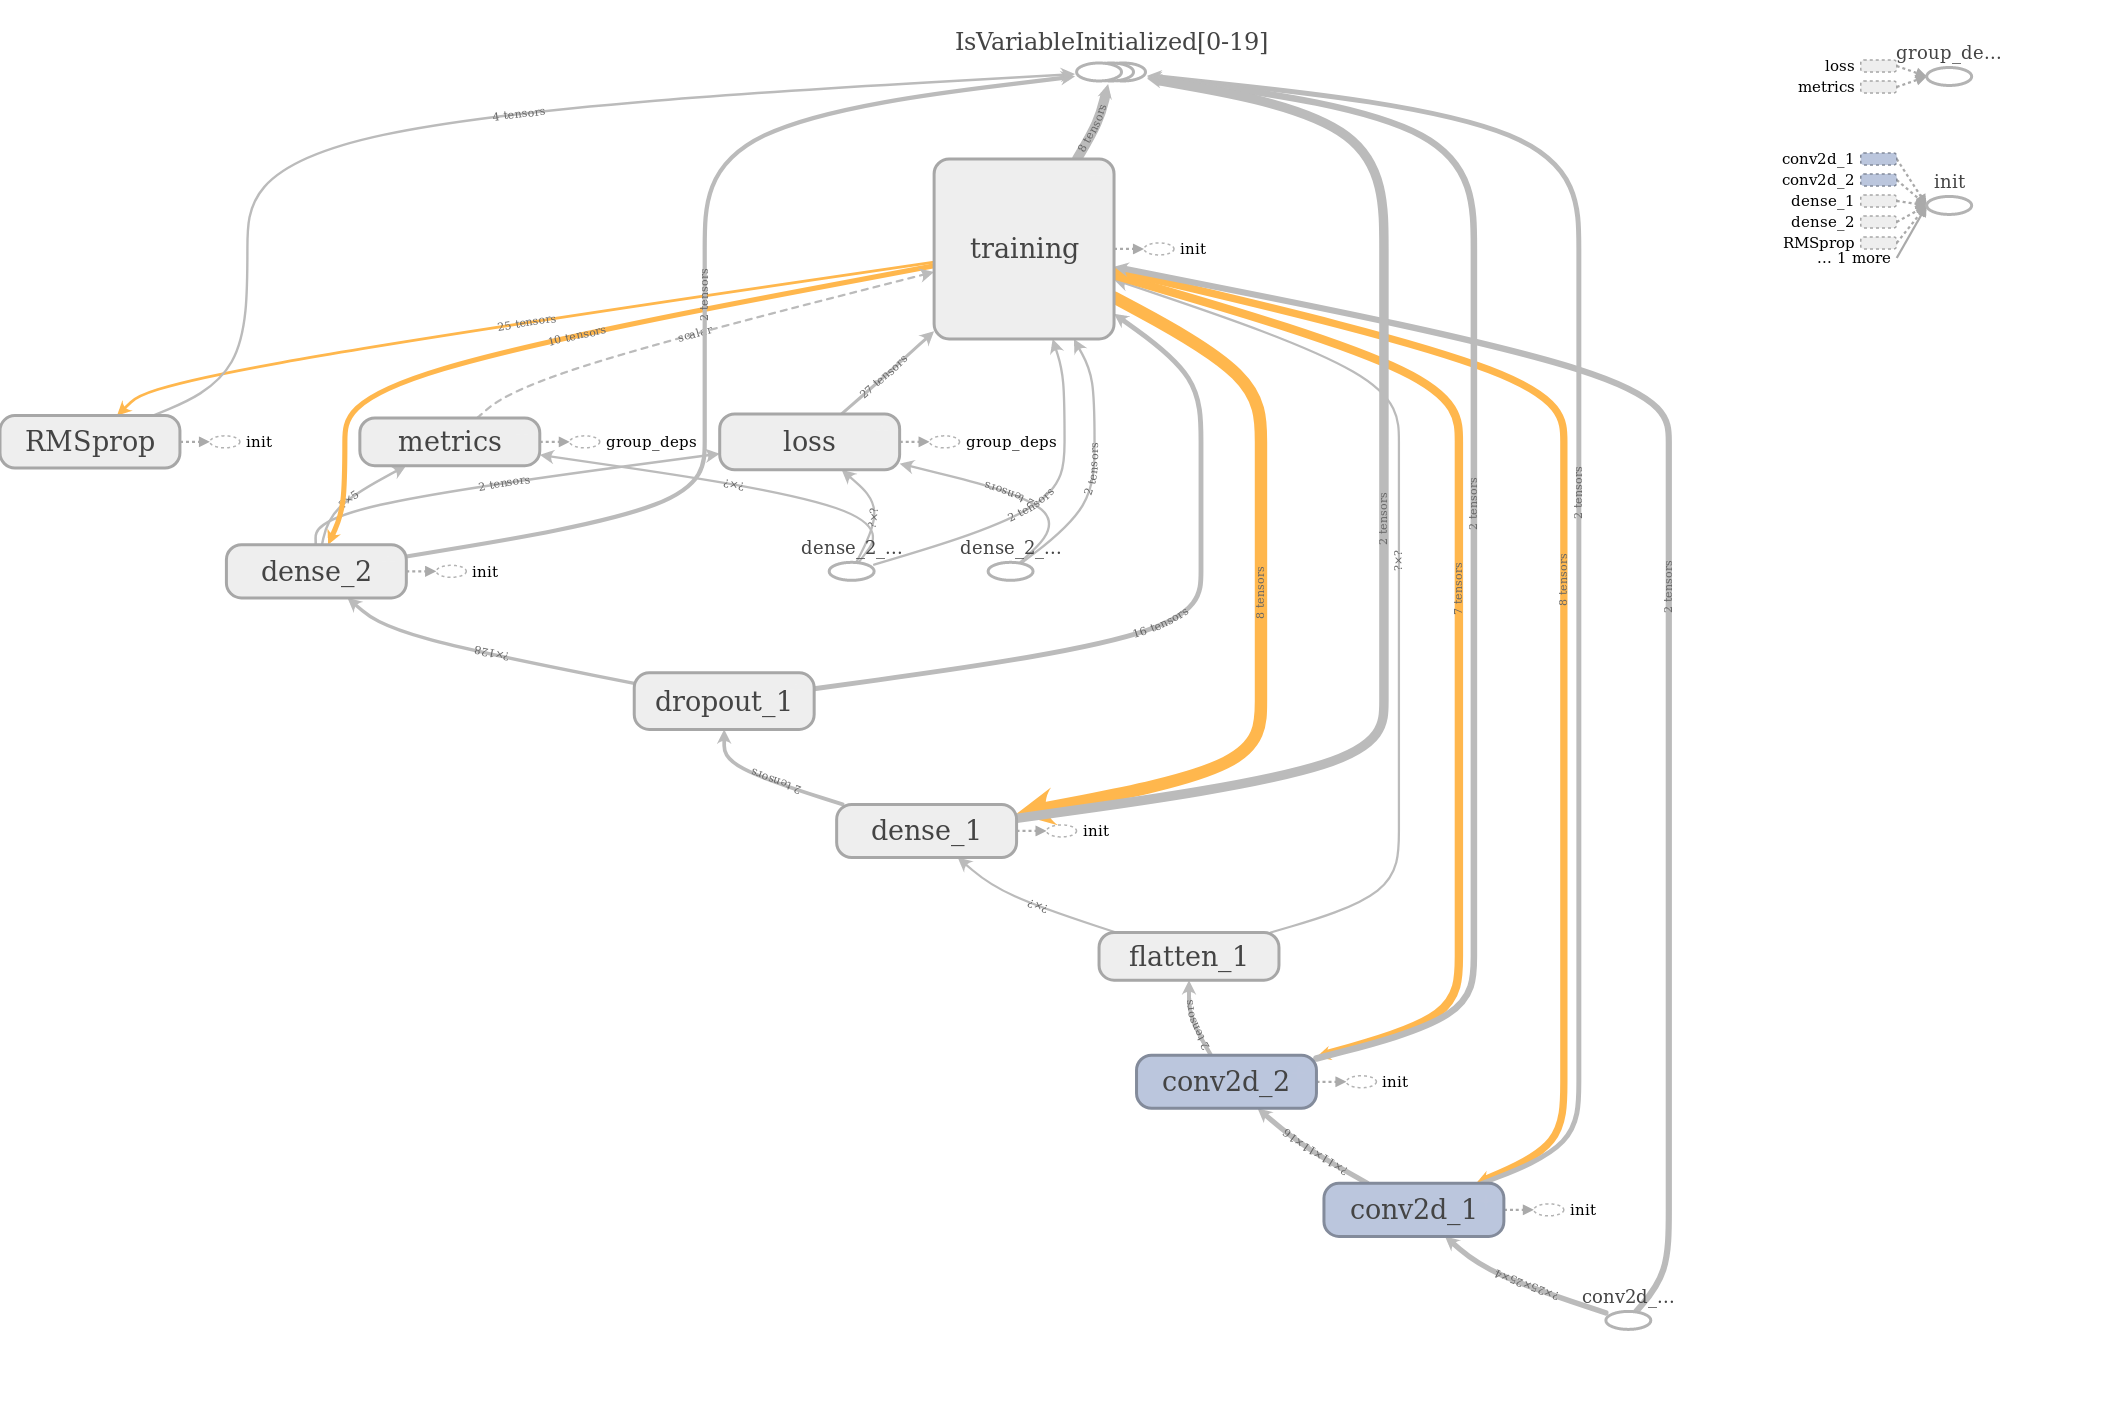
\includegraphics[height=3.5cm,width=\textwidth]{rmsprop_graph.png}
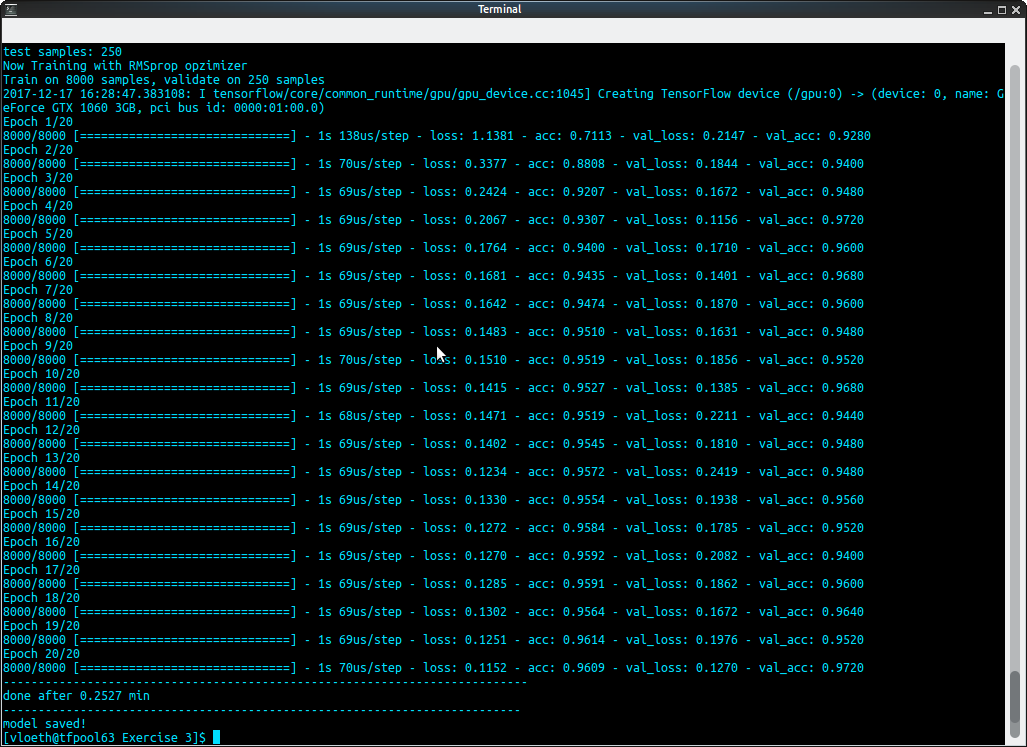
\includegraphics[height=3.5cm,width=\textwidth]{rms_training.png}
\end{minipage}

\begin{minipage}[t]{0.45\textwidth}
\flushleft{Playing with linear output activation}
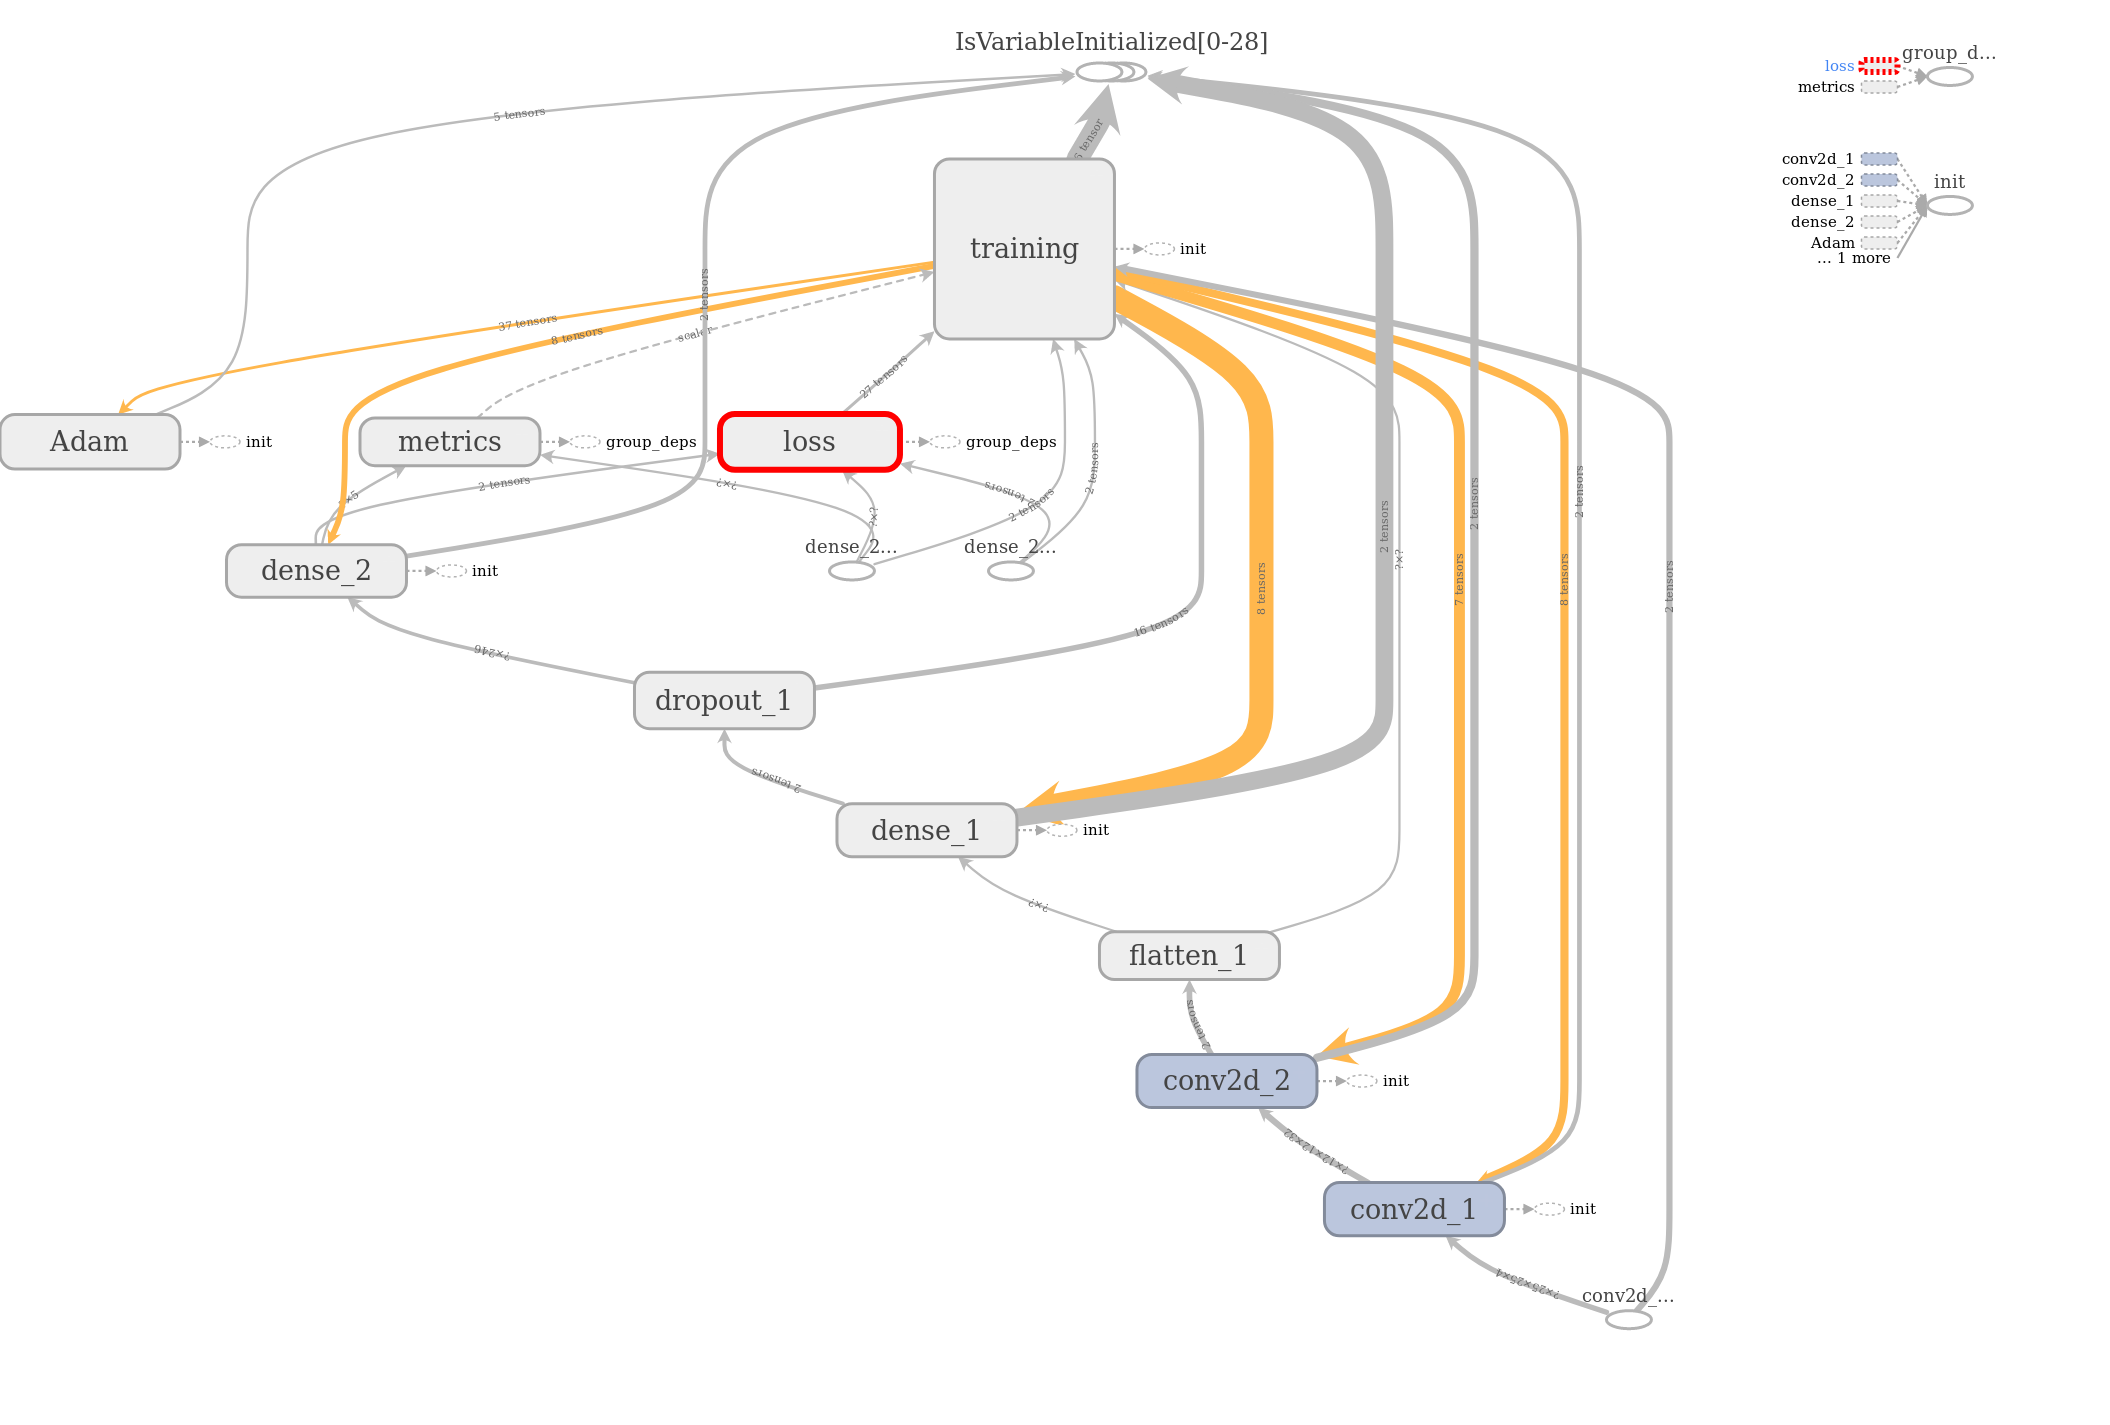
\includegraphics[height=3.5cm,width=\textwidth]{linear_output.png}
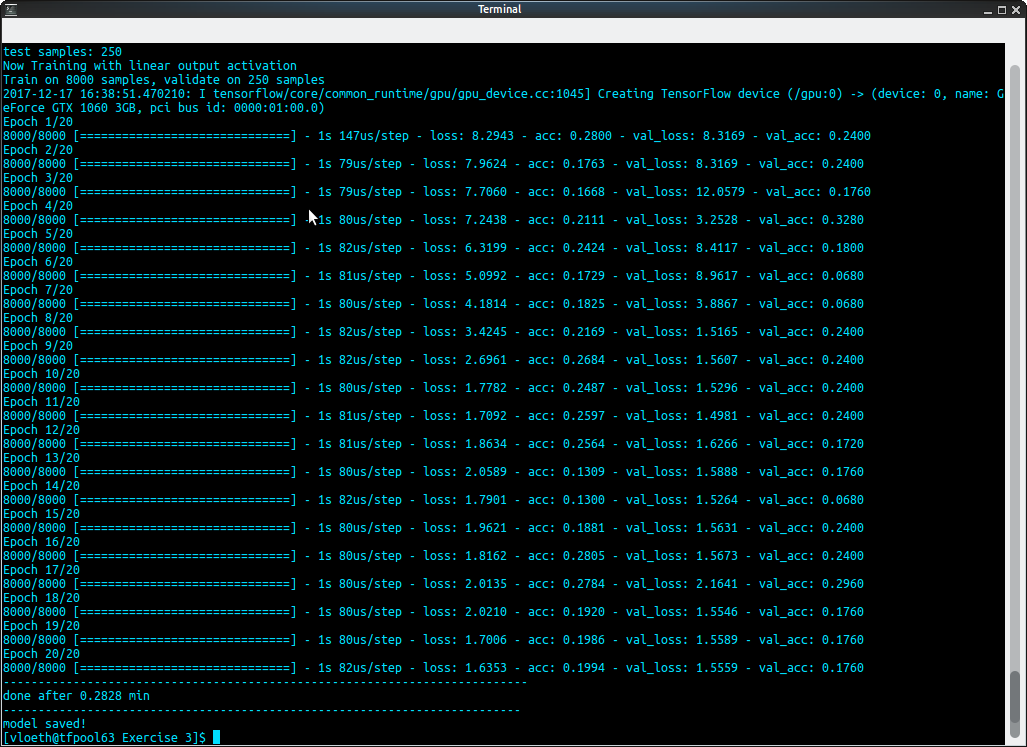
\includegraphics[height=3.5cm,width=\textwidth]{linear_output_training.png}
\end{minipage}
\hfill
\begin{minipage}[t]{0.45\textwidth}
\flushleft{Playing with tanh act. and sigm. output act.}
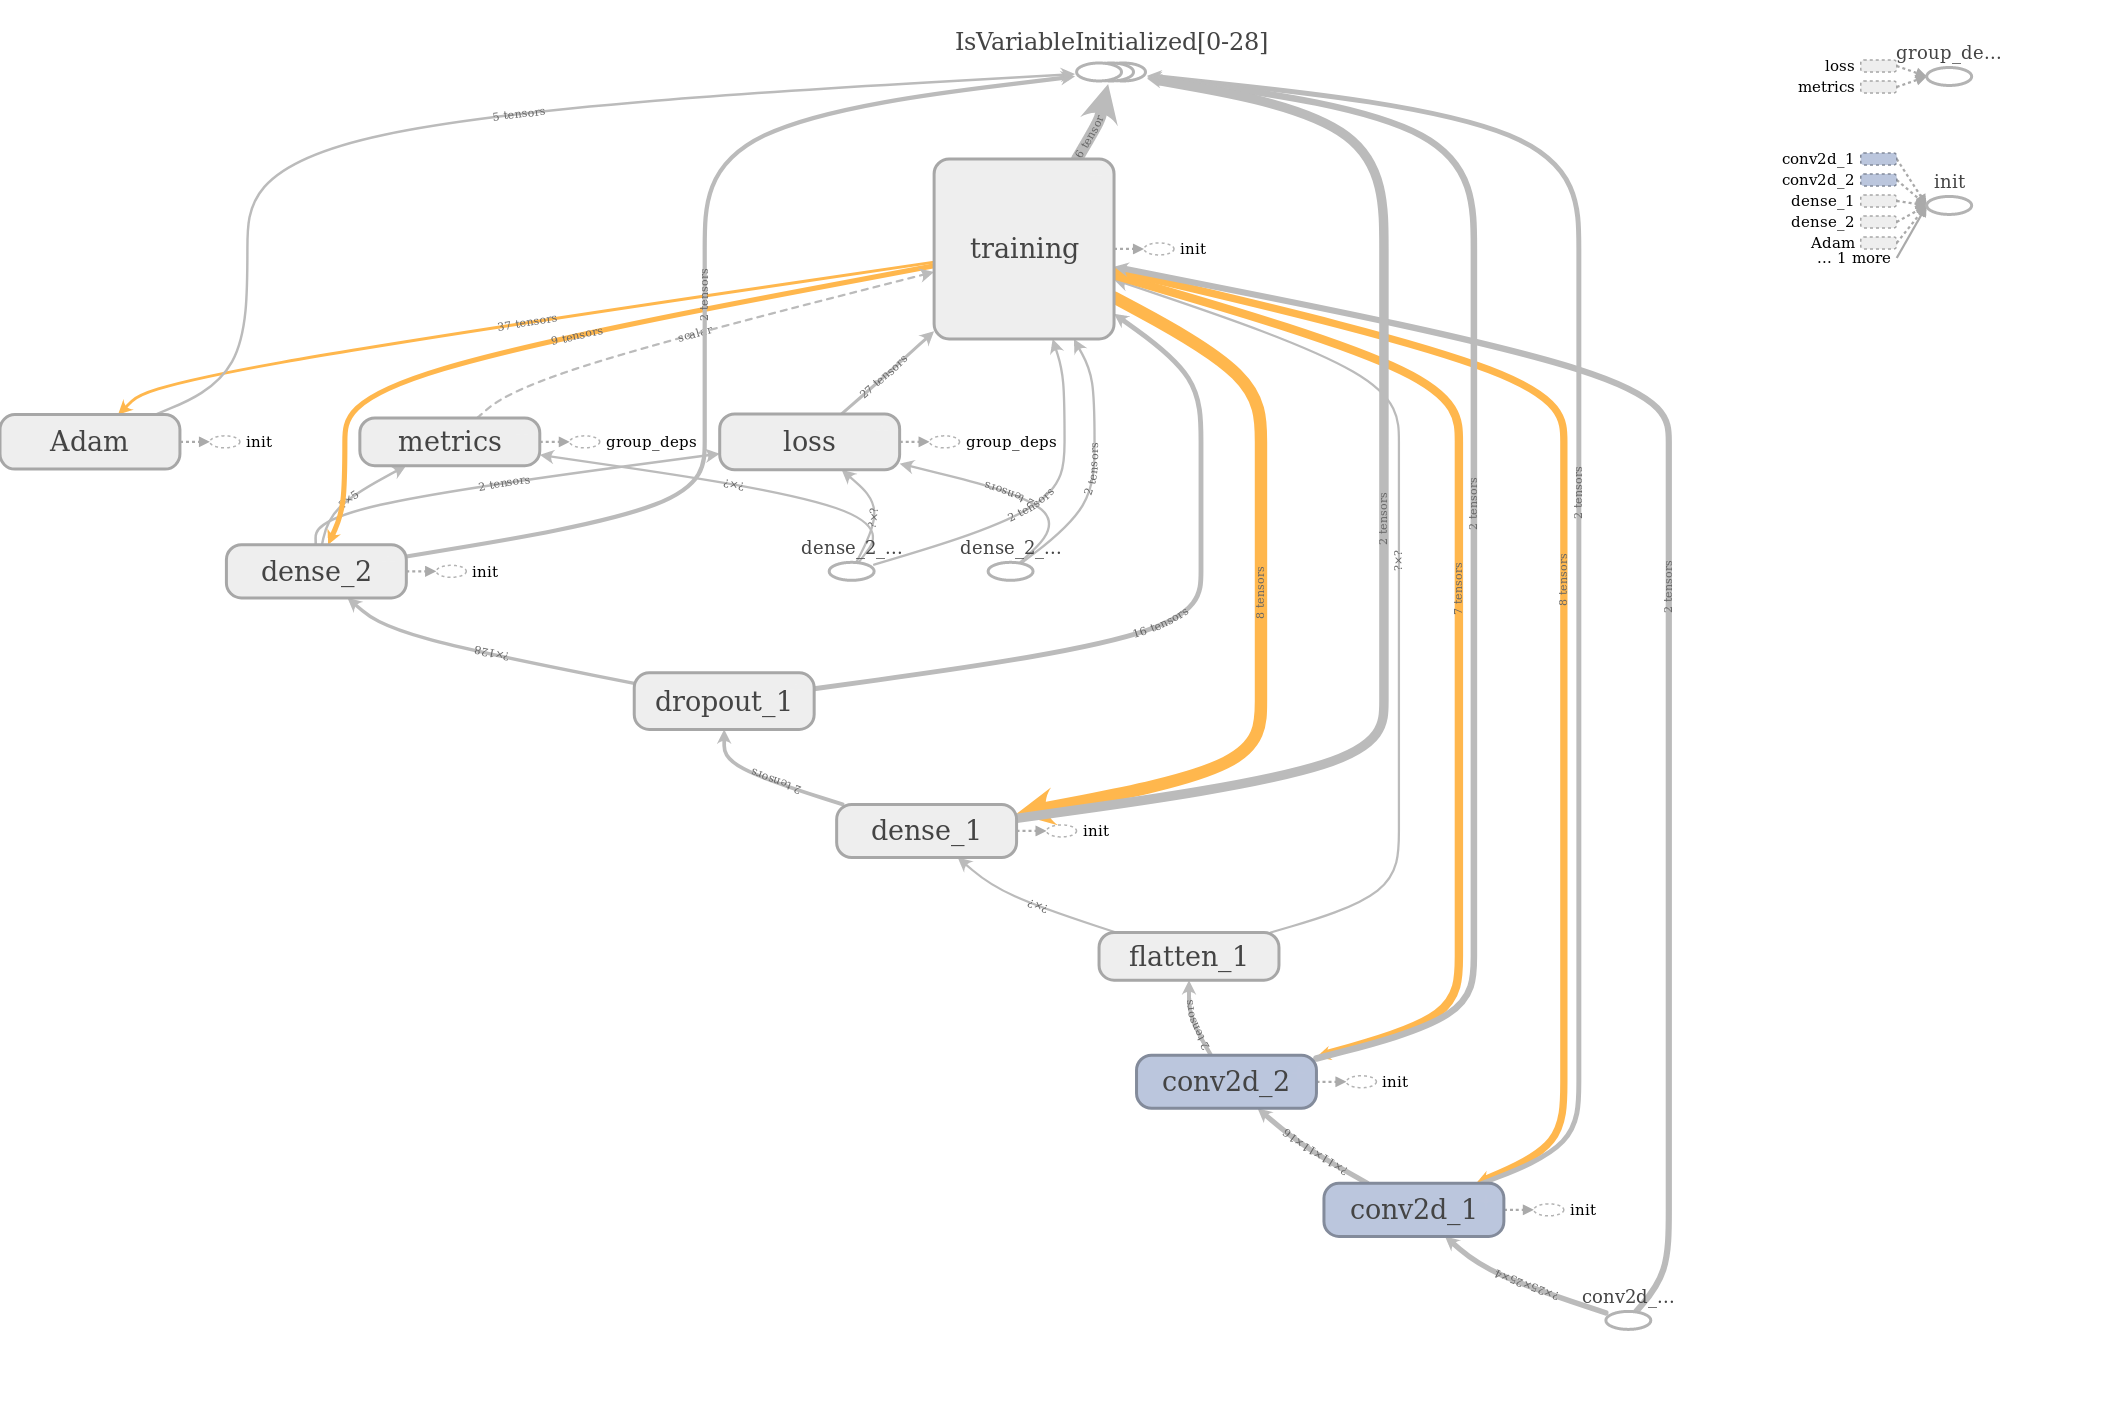
\includegraphics[height=3.5cm,width=\textwidth]{tanh_sigmoid_graph.png}
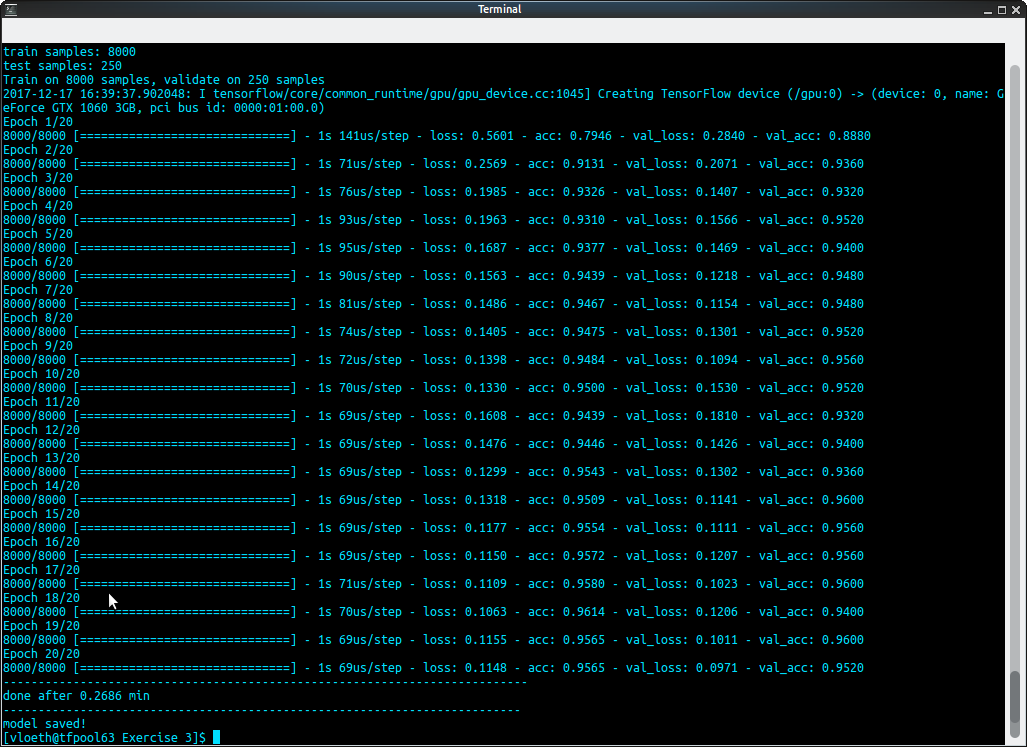
\includegraphics[height=3.5cm,width=\textwidth]{tanh_sigmoid_training.png}
\end{minipage}

\begin{minipage}[t]{0.45\textwidth}
\flushleft{Playing with only fully connected layers}
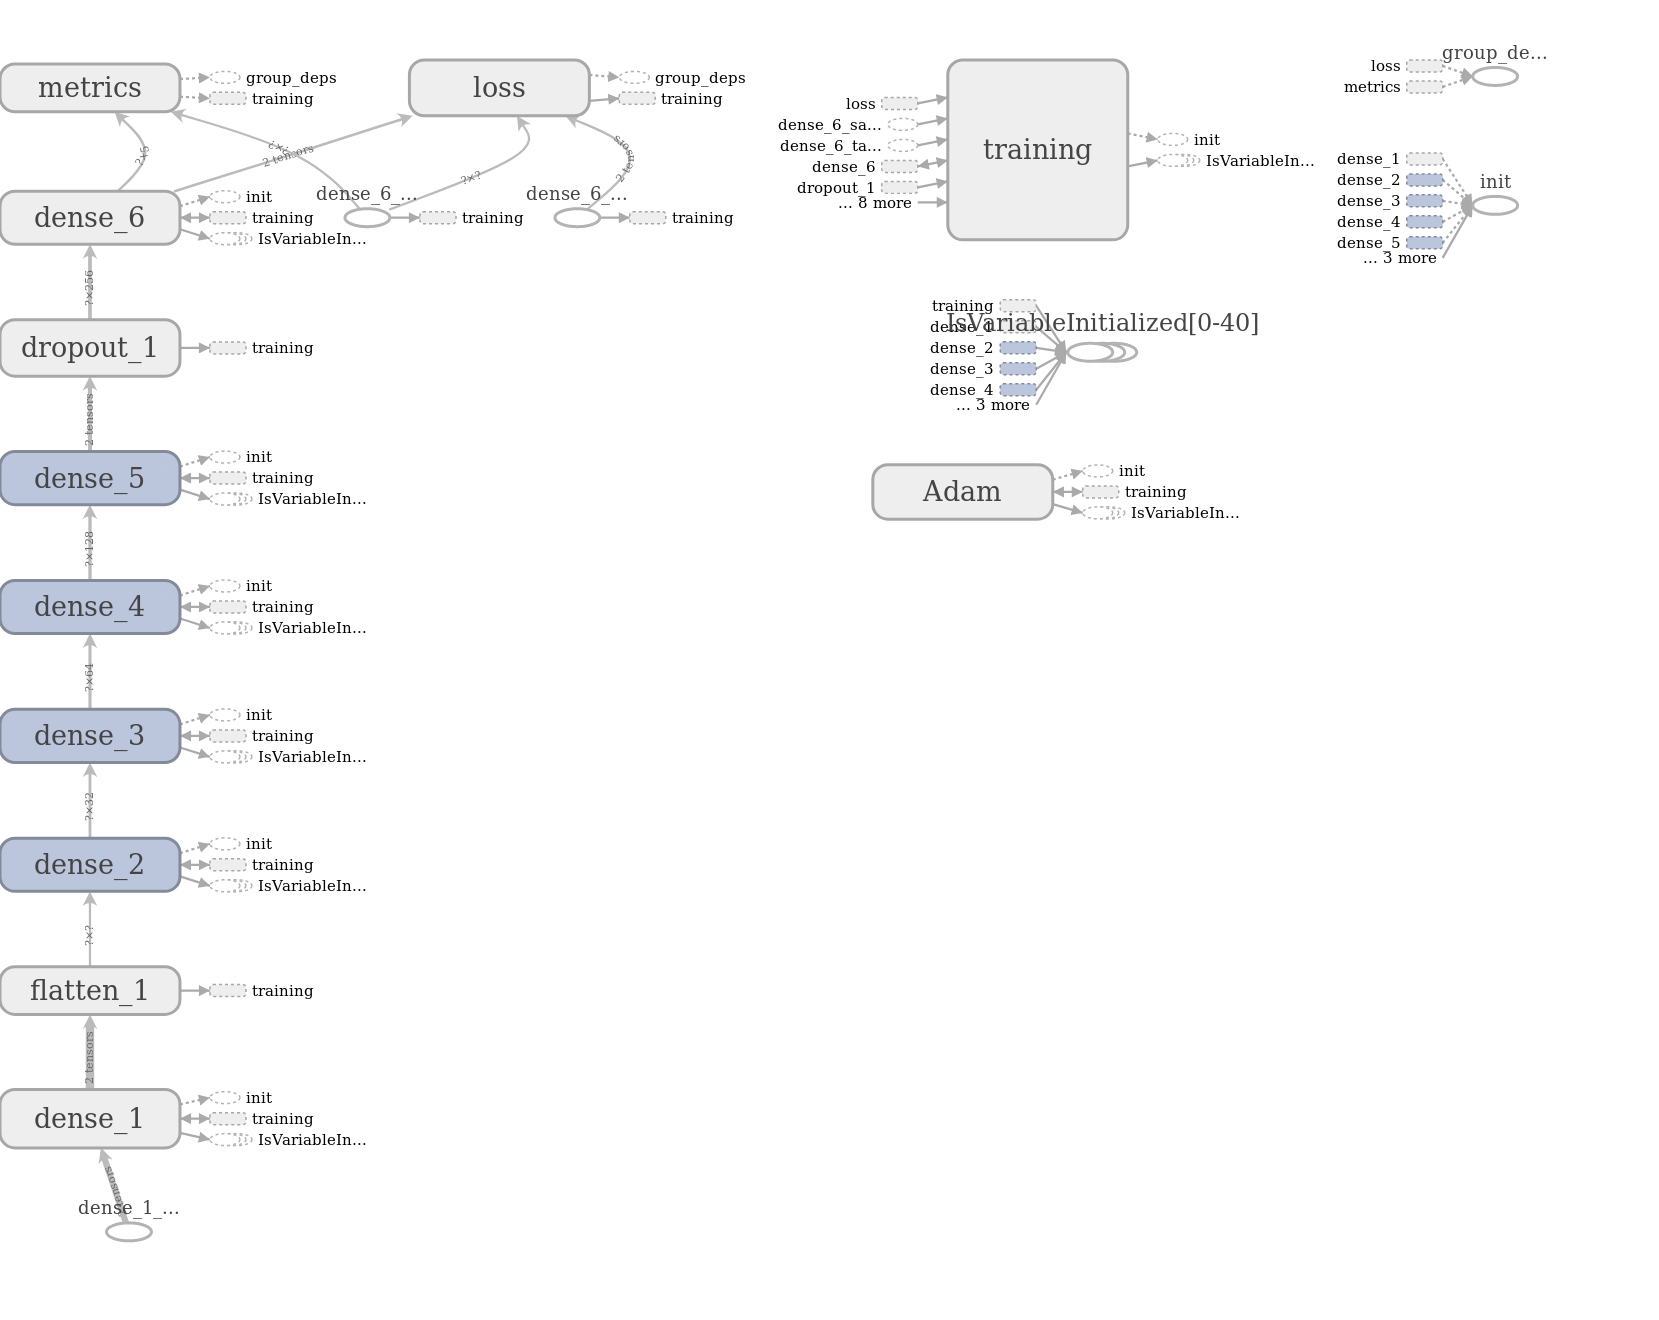
\includegraphics[height=3.5cm,width=\textwidth]{fc_graph.png}
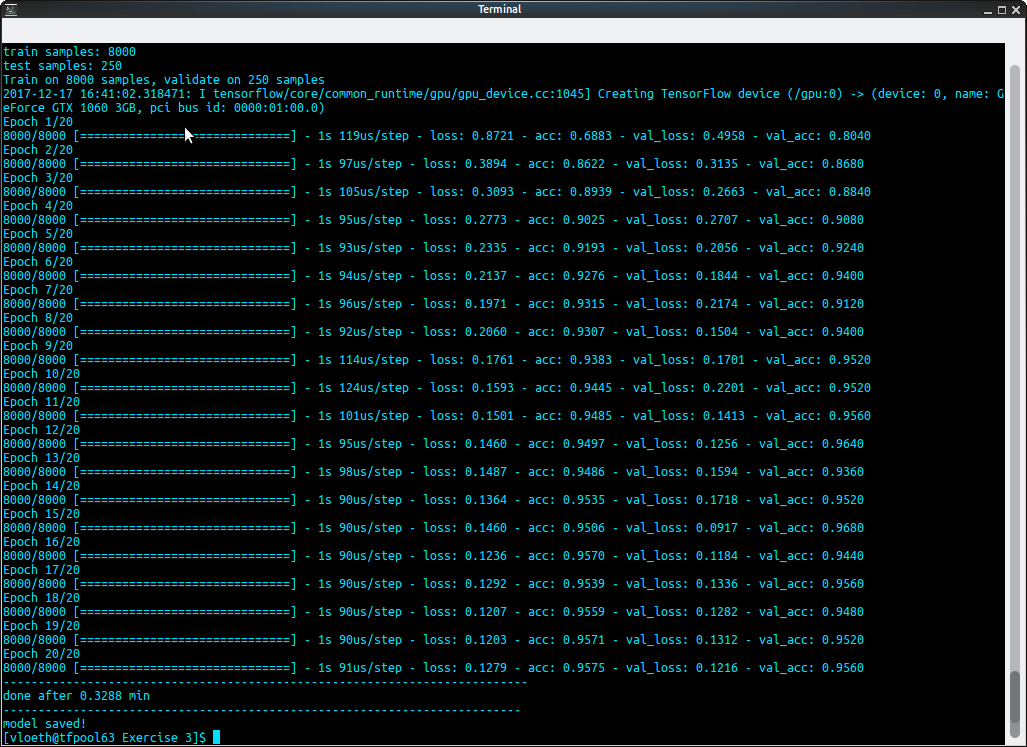
\includegraphics[height=3.5cm,width=\textwidth]{fc_training.png}
\end{minipage}
\hfill


\end{document}